\documentclass[9pt,a4paper]{extarticle}
\usepackage[margin=1.0cm]{geometry}
\usepackage{graphicx}
\usepackage{booktabs}
\usepackage{hyperref}
\usepackage{xcolor}
\hypersetup{colorlinks=true,urlcolor=blue,linkcolor=blue,citecolor=blue}
\setlength{\parindent}{0pt}
\setlength{\parskip}{0.25em}
\pagestyle{empty}
\begin{document}
\begin{center}
{\Large\bfseries Airtel Kenya multi-head message classifier}\\[0.2em]
Christopher Kioko\\
DSA 8401 Applied Machine Learning, Strathmore University
\end{center}

A shared AfroXLMR-base encoder, trained on one Colab T4 with the bottom 8 of 12 layers frozen, scores 10 issue classes, binary sentiment, and ordinal urgency with a CORN head. TF-IDF logistic regression is the CPU baseline. Every number below comes from \texttt{reports/results.json}. Accuracy is the confusion-matrix diagonal divided by \(n\). Macro precision and macro recall are unweighted means of the stored per-class values, so they have no bootstrap interval. Macro-F1, QWK, emergency recall, and the false-emergency rate are the stored estimates and their stored 95\% intervals.

Repository: \url{https://github.com/ChristopherKiokoStrathmore/-DSA8401---ML-CAPSTONE-PROJECT-}\\
Live demo: \url{https://dsa-8401-ml-capstone-project.vercel.app/}\\
API docs (Swagger): \url{https://api-production-09d942cd.up.railway.app/docs}\\
Health: \url{https://api-production-09d942cd.up.railway.app/health}

\begin{center}
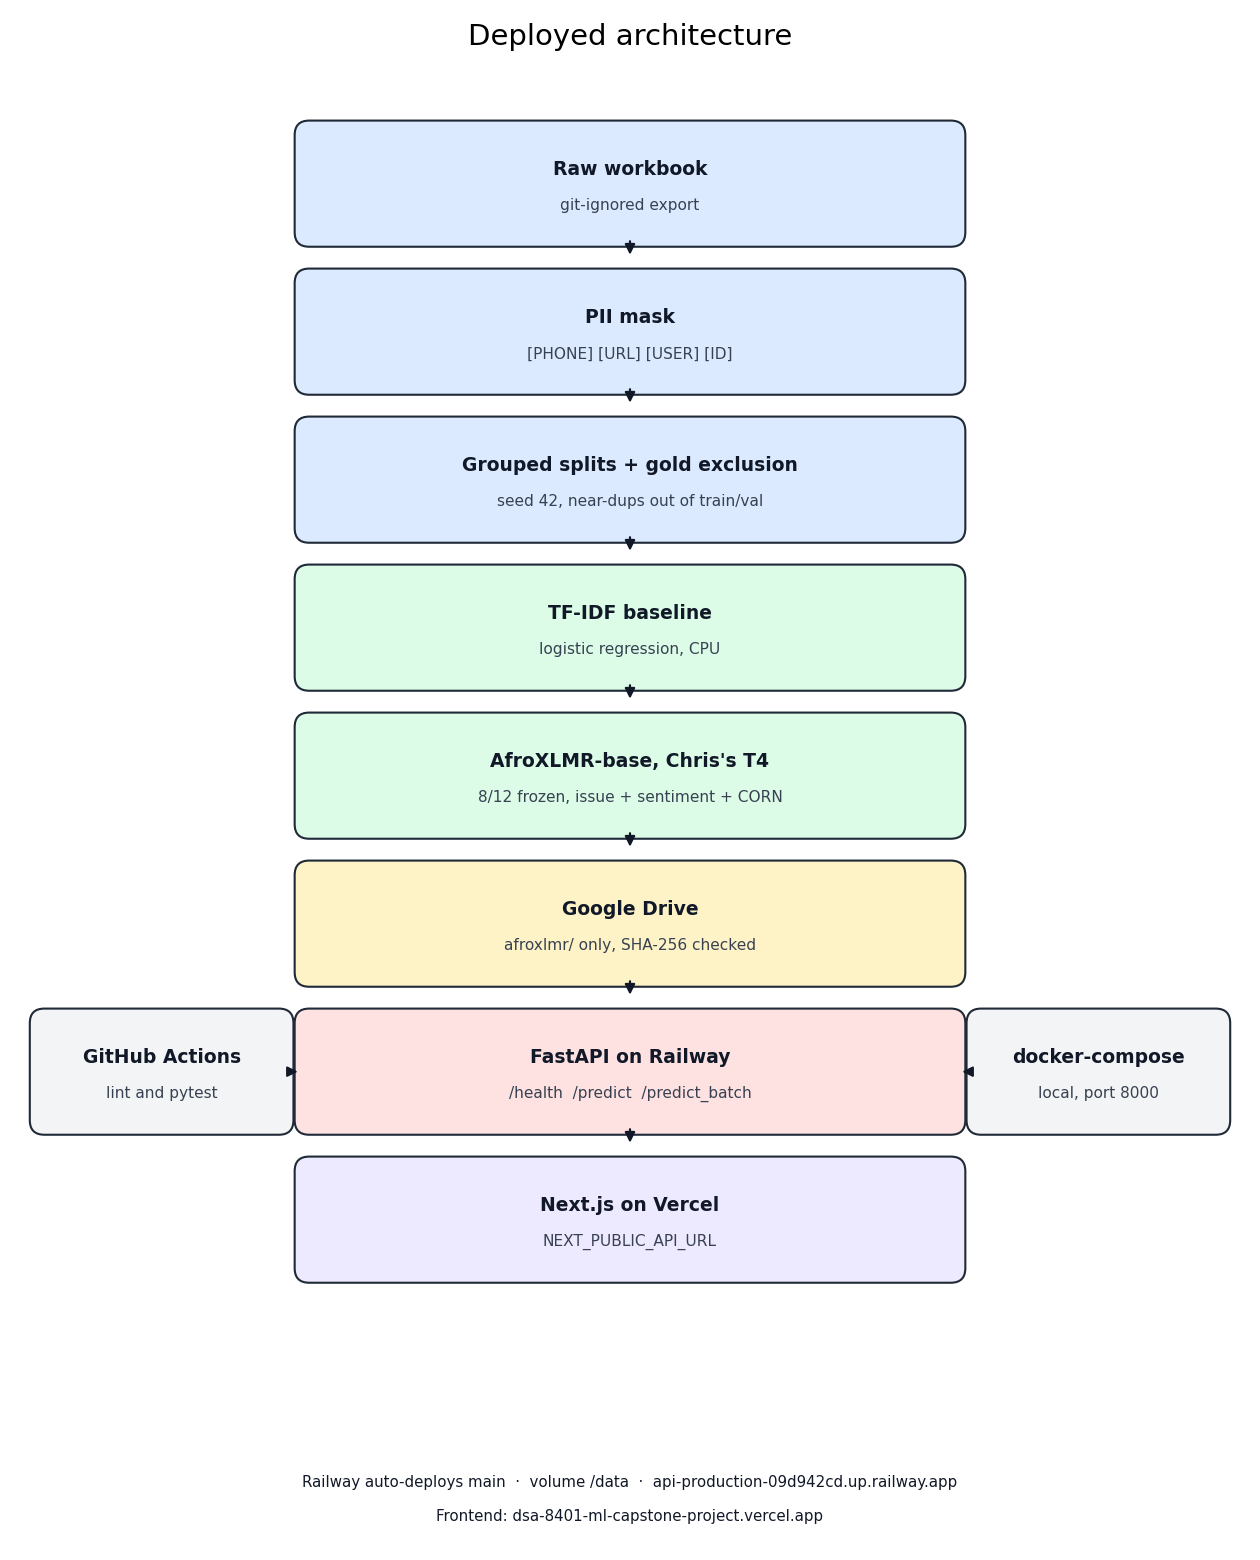
\includegraphics[width=\textwidth]{../docs/architecture-deployed.png}
\end{center}

{\scriptsize
\setlength{\tabcolsep}{2.2pt}
\begin{tabular}{@{}llrlllllll@{}}
\toprule
Head & Model & \(n\) & Acc. & Macro P & Macro R & Macro-F1 (95\% CI) & QWK (95\% CI) & Emerg.\ recall & False-emerg. \\
\midrule
issue & afroxlmr & 224 & 0.772 & 0.652 & 0.669 & 0.656 [0.595, 0.707] &  &  &  \\
issue & tfidf & 224 & 0.723 & 0.701 & 0.625 & 0.636 [0.542, 0.714] &  &  &  \\
sentiment & afroxlmr & 150 & 0.807 & 0.797 & 0.810 & 0.800 [0.727, 0.863] &  &  &  \\
sentiment & tfidf & 150 & 0.767 & 0.755 & 0.764 & 0.758 [0.685, 0.825] &  &  &  \\
urgency & afroxlmr & 120 & 0.717 & 0.687 & 0.689 & 0.687 [0.589, 0.770] & 0.687 [0.567, 0.779] & 0.804 [0.691, 0.906] & 0.145 [0.066, 0.239] \\
urgency & tfidf & 120 & 0.675 & 0.637 & 0.629 & 0.633 [0.526, 0.723] & 0.554 [0.386, 0.691] & 0.667 [0.537, 0.791] & 0.174 [0.083, 0.271] \\
\bottomrule
\end{tabular}

\vspace{0.3em}
Issue per-class precision, recall, and F1. A is AfroXLMR. T is TF-IDF.
\setlength{\tabcolsep}{3.2pt}
\begin{tabular}{@{}lrrrrrrr@{}}
\toprule
Class & \(n\) & A P & A R & A F1 & T P & T R & T F1 \\
\midrule
Airtel\_Money\_Reversal & 4 & 0.000 & 0.000 & 0.000 & 1.000 & 0.250 & 0.400 \\
Airtel\_Money\_Transfer & 19 & 0.654 & 0.895 & 0.756 & 0.667 & 0.842 & 0.744 \\
App\_Rewards & 14 & 1.000 & 0.786 & 0.880 & 0.846 & 0.786 & 0.815 \\
Complaint\_General & 6 & 0.250 & 0.333 & 0.286 & 0.250 & 0.167 & 0.200 \\
Data\_Bundle\_Problems & 22 & 0.792 & 0.864 & 0.826 & 0.615 & 0.727 & 0.667 \\
Network\_Issues & 41 & 0.900 & 0.878 & 0.889 & 0.791 & 0.829 & 0.810 \\
Non\_Actionable & 57 & 0.863 & 0.772 & 0.815 & 0.763 & 0.789 & 0.776 \\
Product\_Enquiry & 20 & 0.650 & 0.650 & 0.650 & 0.571 & 0.400 & 0.471 \\
Router\_WiFi\_5G & 21 & 0.773 & 0.810 & 0.791 & 0.789 & 0.714 & 0.750 \\
SIM\_Line\_Services & 20 & 0.636 & 0.700 & 0.667 & 0.714 & 0.750 & 0.732 \\
\bottomrule
\end{tabular}
}

\vspace{0.35em}
{\small\bfseries Repository map}\\[-0.15em]
{\scriptsize
\setlength{\tabcolsep}{3pt}
\begin{tabular}{@{}l p{12.8cm}@{}}
\toprule
Path & What it is \\
\midrule
\href{https://github.com/ChristopherKiokoStrathmore/-DSA8401---ML-CAPSTONE-PROJECT-/blob/main/README.md}{README.md} & Overview, setup, architecture, and how to reproduce. \\
\href{https://github.com/ChristopherKiokoStrathmore/-DSA8401---ML-CAPSTONE-PROJECT-/blob/main/AI_USE.md}{AI\_USE.md} & Who labelled what, and which tools wrote code. \\
\href{https://github.com/ChristopherKiokoStrathmore/-DSA8401---ML-CAPSTONE-PROJECT-/tree/main/src/capstone}{src/capstone/} & Pipeline, models, and the FastAPI service. \\
\href{https://github.com/ChristopherKiokoStrathmore/-DSA8401---ML-CAPSTONE-PROJECT-/tree/main/config}{config/} & Training config and the weights URL. \\
\href{https://github.com/ChristopherKiokoStrathmore/-DSA8401---ML-CAPSTONE-PROJECT-/blob/main/reports/results.json}{reports/results.json} & Real test metrics for the T4 run. \\
\href{https://github.com/ChristopherKiokoStrathmore/-DSA8401---ML-CAPSTONE-PROJECT-/blob/main/report/report.pdf}{report/report.pdf} & The capstone report. \\
\href{https://github.com/ChristopherKiokoStrathmore/-DSA8401---ML-CAPSTONE-PROJECT-/tree/main/frontend}{frontend/} & Next.js demo that calls this API. \\
\href{https://github.com/ChristopherKiokoStrathmore/-DSA8401---ML-CAPSTONE-PROJECT-/blob/main/Dockerfile}{Dockerfile} & CPU image that serves the API. \\
\href{https://github.com/ChristopherKiokoStrathmore/-DSA8401---ML-CAPSTONE-PROJECT-/blob/main/docker-compose.yml}{docker-compose.yml} & Local API on port 8000. \\
\href{https://github.com/ChristopherKiokoStrathmore/-DSA8401---ML-CAPSTONE-PROJECT-/blob/main/railway.json}{railway.json} & Railway build, healthcheck, and restart. \\
\href{https://github.com/ChristopherKiokoStrathmore/-DSA8401---ML-CAPSTONE-PROJECT-/tree/main/tests}{tests/} & Pytest for the pipeline, models, and API. \\
\href{https://github.com/ChristopherKiokoStrathmore/-DSA8401---ML-CAPSTONE-PROJECT-/tree/main/.github/workflows}{.github/workflows} & GitHub Actions lint and pytest. \\
\href{https://github.com/ChristopherKiokoStrathmore/-DSA8401---ML-CAPSTONE-PROJECT-/tree/main/docs}{docs/} & Rubric, justification, and figures. \\
\bottomrule
\end{tabular}
}
\end{document}
